
% xetex expected
\documentclass[xetex,professionalfont]{beamer}

% we want math
\usepackage{amsmath}

% fixes and extensions to amsmath
\usepackage{mathtools}

% additional math symbols
\usepackage{amssymb}

% good-looking fractions in text via \sfrac
\usepackage{xfrac}

% fix spaces after custom commands (see below for examples)
\usepackage{xspace}

% minted allows for fancy syntax highlighting (requires python with pygments)
% usage:
%   \begin{minted}{python}
%   codeb
%   \end{minted}
% \usepackage{minted}

% better looking tables
% usage:
%   begin with a \toprule, write a single row of column headings,
%   then add \midrule and after the columns of data we finish with \bottomrule
% example:
%   \begin{tabular}{llr} \toprule
%   Animal & Description & Price \midrule
%   cat & foo & 10 \\
%   dog & bar & 20 \\ \bottomrule
%   \end{tabular}
% note that good tables generally neither have vertical rules nor double rules
\usepackage{booktabs}

% system font support (requires xetex or luatex)
\usepackage{fontspec}
\setmonofont[Scale=0.7]{Cousine} % part of ttf-chromeos fonts on Arch

% improve microtypography
\usepackage{microtype}

% multi-language quotes for babel
\usepackage{csquotes}

% easy way to include copyright information
\usepackage{copyrightbox}

% better bibliographies
\usepackage[backend=biber,style=authoryear]{biblatex}

% language support (english,ngerman)
\usepackage[english]{babel}

% plots (part of texlive-pictures)
\usepackage{pgfplots}

% -----------------------------------------------------------------------------

% specify PDF metadata
\hypersetup{pdftitle={CVSP VO - 3D Vision Applications},pdfsubject={},pdfauthor={Christopher Pramerdorfer}}

% copyright font style
\makeatletter\renewcommand{\CRB@setcopyrightfont}{\tiny\color{lightgray}}

% make emph bold
\DeclareTextFontCommand{\emph}{\bfseries}

% use tuwcvl beamer theme
\usetheme{tuwcvl}

% add bib file
\addbibresource{literature.bib}

% plot setup

\pgfplotsset{width=6.5cm,compat=1.11}

\definecolor{darkgreen}{rgb}{0,0.8,0.1}

% -----------------------------------------------------------------------------

% common english abbreviations
\newcommand{\ie}{\mbox{i.e.}\xspace} % i.e.
\newcommand{\eg}{\mbox{e.g.}\xspace} % e.g.
\newcommand{\wrt}{\mbox{wrt.}\xspace} % wrt.

% math - argmin and argmax
\DeclareMathOperator*{\argmin}{arg\,min}
\DeclareMathOperator*{\argmax}{arg\,max}

\DeclareMathOperator*{\Norm}{Norm}
\DeclareMathOperator*{\Uniform}{Uniform}
\DeclareMathOperator*{\Bern}{Bern}

% shortcuts for number ranges
\newcommand{\NN}{\mathbb{N}}
\newcommand{\ZZ}{\mathbb{Z}}
\newcommand{\QQ}{\mathbb{Q}}
\newcommand{\RR}{\mathbb{R}}

% bold vectors
\renewcommand{\vec}[1]{\ensuremath{\mathbf{#1}}}

% vector shortcuts
\newcommand{\va}{\vec{a}}
\newcommand{\vb}{\vec{b}}
\newcommand{\vc}{\vec{c}}
\newcommand{\ve}{\vec{e}}
\newcommand{\vr}{\vec{r}}
\newcommand{\vs}{\vec{s}}
\newcommand{\vt}{\vec{t}}
\newcommand{\vu}{\vec{u}}
\newcommand{\vv}{\vec{v}}
\newcommand{\vw}{\vec{w}}
\newcommand{\vx}{\vec{x}}
\newcommand{\vy}{\vec{y}}
\newcommand{\vz}{\vec{z}}
\newcommand{\vp}{\vec{p}}
\newcommand{\vq}{\vec{q}}
\newcommand{\vn}{\vec{n}}

% bold greek symbols
\newcommand{\bth}{\boldsymbol{\theta}}
\newcommand{\intr}{\boldsymbol{\Lambda}}
\newcommand{\trans}{\mathcal{T}}

% -----------------------------------------------------------------------------

\title{Computer Vision Systems Programming VO}
\subtitle{3D Vision Applications}
\author{Christopher Pramerdorfer}
\institute{Computer Vision Lab, Vienna University of Technology}

\begin{document}

% -----------------------------------------------------------------------------

\begin{frame}
\maketitle
\end{frame}

% -----------------------------------------------------------------------------

\begin{frame}
\frametitle{Topics}

CV applications utilizing scene geometry (3D data)
\begin{itemize}
	\item Focus on those based on Kinect % because it is so popular
\end{itemize}

\bigskip
\begin{center}
    \copyrightbox[b]
    {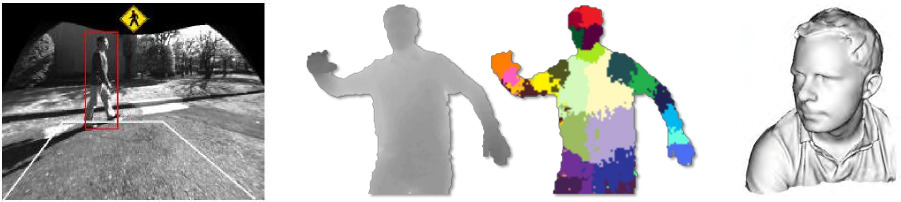
\includegraphics[width=10cm]{figures/intro-collage.jpg}}
    {\centering Images by Ryuzo Okada, \cite{shotton2011}, \cite{newcombe2011}}
\end{center}

\end{frame}

% -----------------------------------------------------------------------------

\begin{frame}
\frametitle{3D Reconstruction}

\begin{center}
    \copyrightbox[b]
    {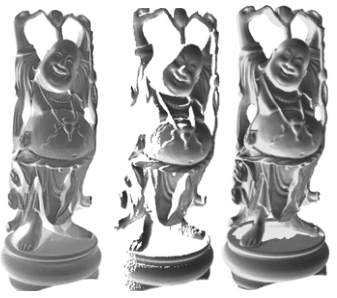
\includegraphics[width=6cm]{figures/3d-reco-tsdf.png}} % photo of the original statue, model from single range scan, model from combined range scans
    {\centering Images from \cite{curless1996}}
\end{center}

\end{frame}

% -----------------------------------------------------------------------------

\begin{frame}
\frametitle{3D Reconstruction}

Construction of accurate 3D models from range data
\begin{itemize}
	\item Usually involves combing multiple point clouds % because there are holes due to occlusions / data from point clouds / depth maps / disparity maps ... these are treated as equal because we can map between them ... se previous slide set
\end{itemize}

\bigskip
Accomplished in two steps % these can be alternating, e.g. with kinect fusion
\begin{itemize}
	\item Align range data (map to common coordinate system)
	\item Merge range data in a way that minimizes errors % otherwise we could just concatenate the points
\end{itemize}

\bigskip
Often followed by surface reconstruction % many reconstruction methods result in a point cloud, but in many applications we want triangle meshes

\end{frame}

% -----------------------------------------------------------------------------

\begin{frame}
\frametitle{3D Reconstruction}
\framesubtitle{Range Data Alignment -- Iterative Closest Points}

Popular method for aligning two point clouds $\{\vr\}$, $\{\vs\}$
\begin{itemize}
	\item Goal is to find parameters $\bth$ of some transformation $\trans$ % note that this again fits our model-based CV approach discussed earlier. we take one cloud as the reference (w) and one as measurements (x), and T(x;theta) is our model that relates these two
	\item Usually assuming a rigid transformation % thats a translation + rotation, which is what we get when observing the same object from different views
\end{itemize}

\bigskip
\begin{center}
    \copyrightbox[b]
    {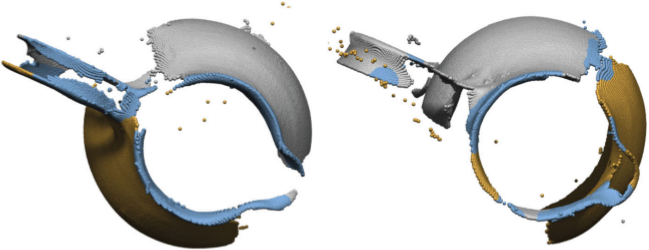
\includegraphics[width=6.5cm]{figures/pot-clouds.png}} % the images are from a different paper, but including them here because they look good
    {\centering Images from \cite{aiger2008}}
\end{center}

\end{frame}

% -----------------------------------------------------------------------------

\begin{frame}
\frametitle{3D Reconstruction}
\framesubtitle{Range Data Alignment -- Iterative Closest Points}

Algorithm iterates between
\begin{itemize}
	\item Finding point correspondences based on distance, $\{(r_n,s_n)\}_n$ % s_i corresponds to r_j if no their distance is below t and if no other s is closer to r_j
	\item Finding the $\bth$ that minimizes $\sum_n\lVert\vr_{r_n}-\trans(\vs_{s_n};\bth) \rVert_2^2$ % this denotes the squares l2 norm ... least squares problem, as the solution to the ML estimate assuming constant additive Gaussian noise ... the minimum can be found in closed form if T is linear (like with a rigid transformation) ... but we still need an iterative approach because the correspondences are erroneous
\end{itemize}

\bigskip
Converges towards a local minimum
\begin{itemize}
	\item Requires good initial estimate of $\bth$ % ICP is a typical example of an iterative optimization problem. as such, it is crucial that the initial parameter estimates are close to the global minimum, otherwise the optimization gets stuck in a local minimum. we have discussed this before, and it is nicely visible in the below video.
\end{itemize}

\bigskip
\begin{center}
	\url{https://www.youtube.com/watch?v=ii2vHBwlmo8}
\end{center}

% note that ICP always operates on two point clouds. what if we want to align more than two? simply chaining ICP quickly produces bad results because it accumulates errors. but there are some alternatives, like global optimization or Kinect Fusion's approach (see below)

\end{frame}

% -----------------------------------------------------------------------------

\begin{frame}
\frametitle{3D Reconstruction}
\framesubtitle{Range Data Merging -- TSDF Fusion}

Truncated signed distance functions (TSDFs)
\begin{itemize}
	\item Similar to distance transforms in 3D (0 = surface)
	\item But distances are signed, measured along view rays 
\end{itemize}

\begin{center}
    \copyrightbox[b]
    {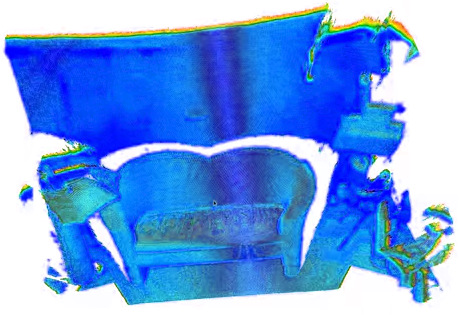
\includegraphics[width=5cm]{figures/tsdf.jpg}}
    {\centering Image from \url{https://www.youtube.com/watch?v=AjjSZufyprU}}
\end{center}

\end{frame}

% -----------------------------------------------------------------------------

\begin{frame}
\frametitle{3D Reconstruction}
\framesubtitle{Range Data Merging -- TSDF Fusion}

Merged data = weighted average over aligned TSDF voxels % this leads to an optimal combination in a least sqaure sense under some simplified assumptions, see the paper
\begin{itemize}
	\item Weights based on \eg object distance, angle
\end{itemize}

\begin{center}
    \copyrightbox[b]
    {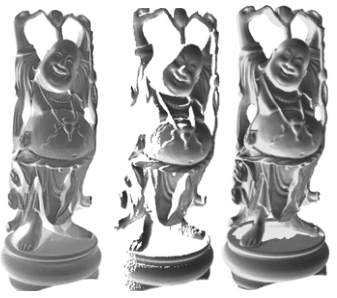
\includegraphics[width=5cm]{figures/3d-reco-tsdf.png}} % photo of the original statue, model from single range scan, model from combined range scans
    {\centering Images from \cite{curless1996}}
\end{center}

\end{frame}

% -----------------------------------------------------------------------------

\begin{frame}
\frametitle{3D Reconstruction}
\framesubtitle{Kinect Fusion}

Temporal fusion of Kinect depth maps

\bigskip
Based on the above methods (ICP \& TSDF fusion)
\begin{itemize}
	\item But $\{\vr\}$ is synthesized from merged model
	\item Suppresses alignment error accumulation % see the comment above ... alignment errors propagate
\end{itemize}

\begin{center}
    \copyrightbox[b]
    {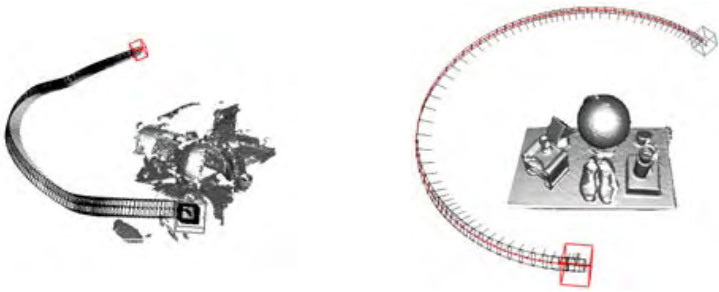
\includegraphics[width=6cm]{figures/kinect-fusion-tracking.jpg}}
    {\centering Images from \cite{newcombe2011}}
\end{center}

\end{frame}

% -----------------------------------------------------------------------------

\begin{frame}
\frametitle{3D Reconstruction}
\framesubtitle{Kinect Fusion}

\begin{center}
	\url{https://www.youtube.com/watch?v=quGhaggn3cQ}
\end{center}

\begin{center}
    \copyrightbox[b]
    {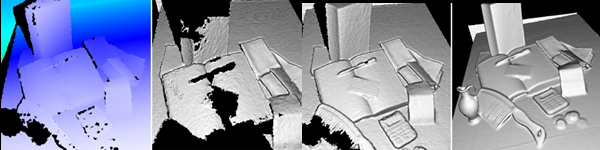
\includegraphics[width=10cm]{figures/kinect-fusion.png}}
    {\centering Images from \url{microsoft.com}}
\end{center}

\end{frame}

% -----------------------------------------------------------------------------

\begin{frame}
\frametitle{3D Reconstruction}
\framesubtitle{Surface Reconstruction}

Reconstruction of surface mesh from point cloud
\begin{itemize}
    \item Results in a (locally) watertight 3D model % watertight = object surface is closed, not just a bunch of points in space
    \item Allows for further processing (e.g.\ texturing)
\end{itemize}

\bigskip
\begin{center}
    \copyrightbox[b]
    {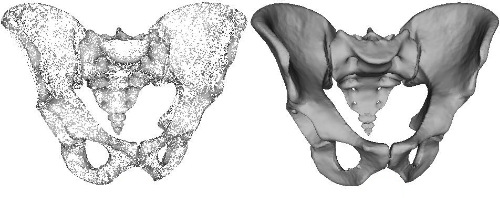
\includegraphics[width=6cm]{figures/hip-points-surface.jpg}}
    {\centering Image from \cite{kazhdan2005}}
\end{center}

\end{frame}

% -----------------------------------------------------------------------------

\begin{frame}
\frametitle{3D Reconstruction}
\framesubtitle{Surface Reconstruction}

Correction of point cloud errors
\begin{itemize}
    \item Noise, outliers, alignment errors, missing data
\end{itemize}

\bigskip
\begin{center}
    \copyrightbox[b]
    {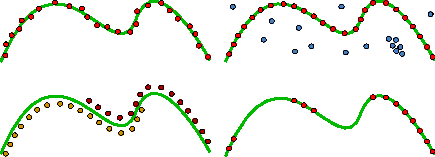
\includegraphics[width=7cm]{figures/point-cloud-errors}}
    {\centering Image adapted from \cite{berger2014}} % nice paper on current surface reconstruction methods
\end{center}

\end{frame}

% -----------------------------------------------------------------------------

\begin{frame}
\frametitle{3D Reconstruction}
\framesubtitle{Surface Reconstruction -- Poisson Surface Reconstruction}

\begin{center}
    \copyrightbox[b]
    {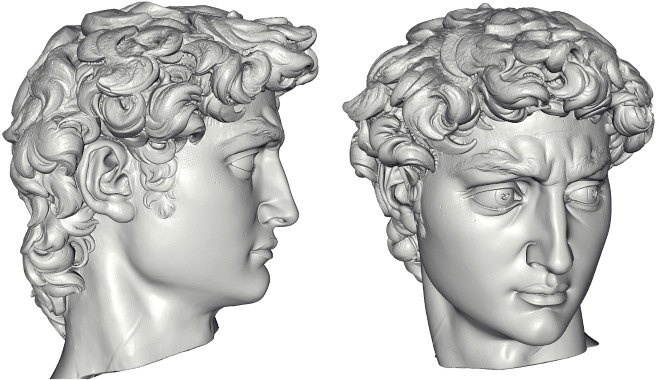
\includegraphics[width=8cm]{figures/psr-david.jpg}}
    {\centering Images from \cite{kazhdan2006}}
\end{center}

\end{frame}

% -----------------------------------------------------------------------------

\begin{frame}
\frametitle{3D Reconstruction}
\framesubtitle{Surface Reconstruction -- Poisson Surface Reconstruction}

Define $\chi(\vx)=1$ if $\vx$ inside the object, $0$ otherwise
\begin{itemize}
    \item Surface is at $\chi(\cdot)=0.5$
    \item $\nabla\chi$ equals surface normal near surface, $0$ otherwise
\end{itemize}

\bigskip
\begin{center}
    \copyrightbox[b]
    {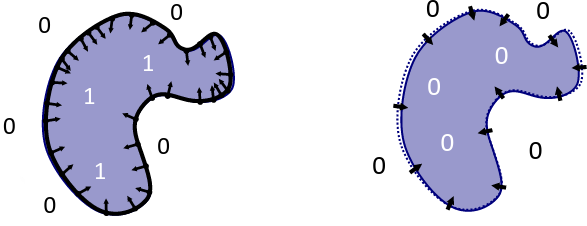
\includegraphics[width=7cm]{figures/psr-indicator.png}} % left: chi, right: nabla chi
    {\centering Images from Gotsman \& Kazhdan's slides}
\end{center}

\end{frame}

% -----------------------------------------------------------------------------

\begin{frame}
\frametitle{3D Reconstruction}
\framesubtitle{Surface Reconstruction -- Poisson Surface Reconstruction}

Regard oriented points $\{(\vx,\vn)\}$ as samples from $\nabla\chi$, $\nabla\chi(\vx)=\vn$ % oriented point = point x with normal vector n ... normals must be estimated in a preprocessing step
\begin{itemize}
    \item Points define vector field $\mathcal{V}$ that corresponds to $\nabla\chi$ % put simply, V is obtained by applying a smoothing filter to the point cloud
    \item Sought $\chi$ minimizes $\lVert\nabla\chi-\mathcal{V}\rVert$ % check out the paper if interested in how this is done
\end{itemize}

\bigskip
\begin{center}
    \copyrightbox[b]
    {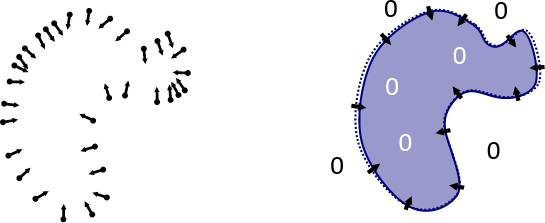
\includegraphics[width=7cm]{figures/psr-vector-field.png}} % left: V at point locations, right: nabla chi
    {\centering Images from Gotsman \& Kazhdan's slides}
\end{center}

\end{frame}

% -----------------------------------------------------------------------------

\begin{frame}
\frametitle{3D Reconstruction}
\framesubtitle{Surface Reconstruction -- Poisson Surface Reconstruction}

Once $\chi$ is known, the isosurface $\chi(\cdot)=0.5$ can be extracted
\begin{itemize}
    \item Using marching cubes, for example
\end{itemize}

\bigskip
\begin{center}
    \copyrightbox[b]
    {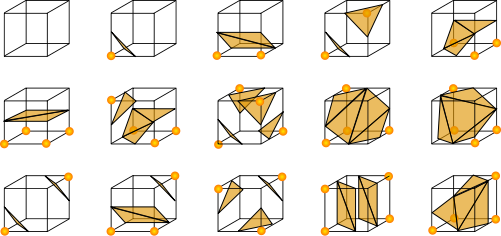
\includegraphics[width=7cm]{figures/marching-cubes.png}}
    {\centering Images from \url{wikipedia.org}}
\end{center}

\end{frame}

% -----------------------------------------------------------------------------

\begin{frame}
\frametitle{3D Reconstruction}
\framesubtitle{Software -- Point Cloud Library (PCL)}

C++ open-source library for point cloud processing\\\medskip
Includes implementations of the above methods

\bigskip
\begin{center}
    \copyrightbox[b]
    {
\includegraphics[width=6cm]{figures/pcl-logo.png}}
    {\centering Image from \url{pointclouds.org}}
\end{center}

\end{frame}

% -----------------------------------------------------------------------------

\begin{frame}
\frametitle{3D Reconstruction}
\framesubtitle{Application Fields -- Cultural Heritage} % only a small selection of course

Preservation of physical artifacts

\bigskip
\begin{center}
    \copyrightbox[b]
    {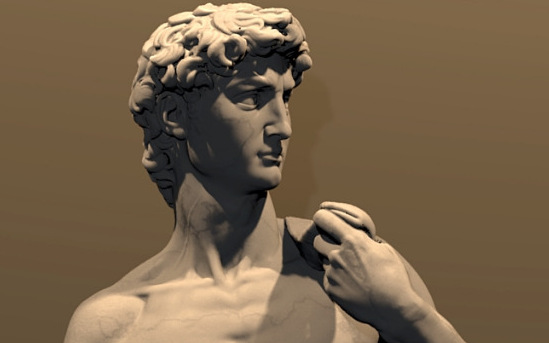
\includegraphics[width=6cm]{figures/david-model.jpg}} % rendering of a 3d model of Michelangelo's David, obtained using a laser scanner. there are now reconstruction methods that lead to a similar accuracy while using only high resolution images
    {\centering Image from \cite{levoy2000}}
\end{center}

\end{frame}

% -----------------------------------------------------------------------------

\begin{frame}
\frametitle{3D Reconstruction}
\framesubtitle{Application Fields -- Virtual and Augmented Reality}

Project Tango

\bigskip
\begin{center}
    \copyrightbox[b]
    {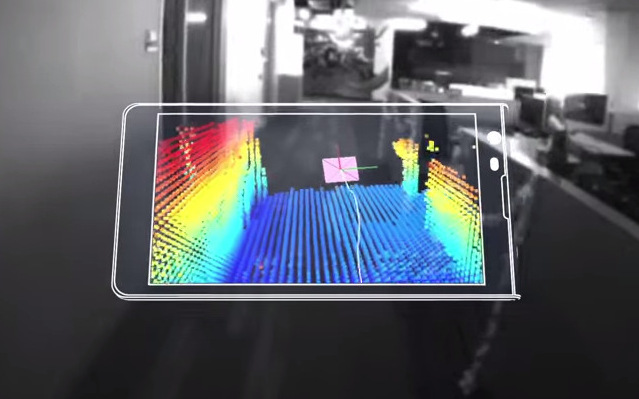
\includegraphics[width=7cm]{figures/project-tango.jpg}}
    {\centering Image from \url{https://www.youtube.com/watch?v=Qe10ExwzCqk}}
\end{center}

\end{frame}

% -----------------------------------------------------------------------------

\begin{frame}
\frametitle{Person Detection}

3D data enables reliable person detection
\begin{itemize}
    \item Robust motion detection
	\item Distinctive, invariant features % depends on the features of course, but the source data (3D points in world coords) are
\end{itemize}

\begin{center}
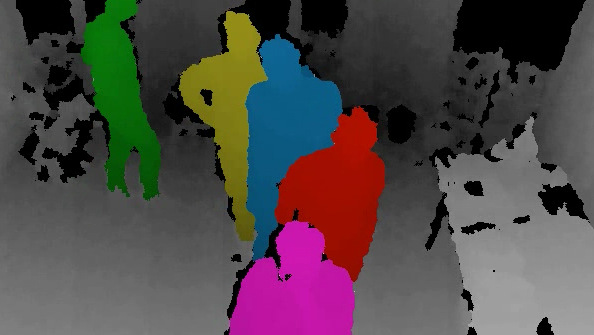
\includegraphics[width=6.5cm]{figures/person-detection.jpg}
\end{center}

\end{frame}

% -----------------------------------------------------------------------------

\begin{frame}
\frametitle{Person Detection}
\framesubtitle{Motion Detection}

Reliable motion detection via background subtraction
\begin{itemize}
    \item Measurements represent object distances
    \item Not affected by illumination, clothing, shadows % these are major problems with normal intensity or color images. of course, the data might be effected if the sensor that generates the distance measurements is affected, but we assume a reliable depth stream here (from a Kinect, for example)
\end{itemize}

\begin{center}
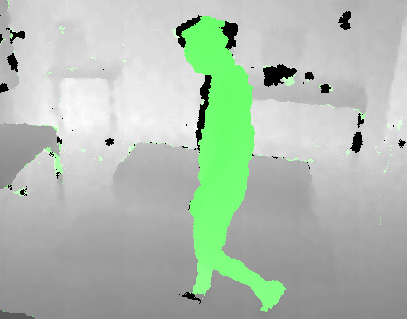
\includegraphics[width=5cm]{figures/fearless-depth.png}
\end{center}

\end{frame}

% -----------------------------------------------------------------------------

\begin{frame}
\frametitle{Person Detection}
\framesubtitle{Features}

Scene geometry allows for distinctive, invariant features
\begin{itemize}
    \item Object size, extent, volume, shape, ... % if we know the extrinsics
\end{itemize}

\bigskip
More on object detection later

\end{frame}

% -----------------------------------------------------------------------------

\begin{frame}
\frametitle{Person Detection}
\framesubtitle{Applications -- Breaking Assistance}

\begin{center}
	\url{https://www.youtube.com/watch?v=oU4XQvxO10k} % the Mercedes also uses radar for this, for longer range and probably during nighttime. it's also just one example, must manufacturers now have some form of this in their premium models
\end{center}

\begin{center}
    \copyrightbox[b]
    {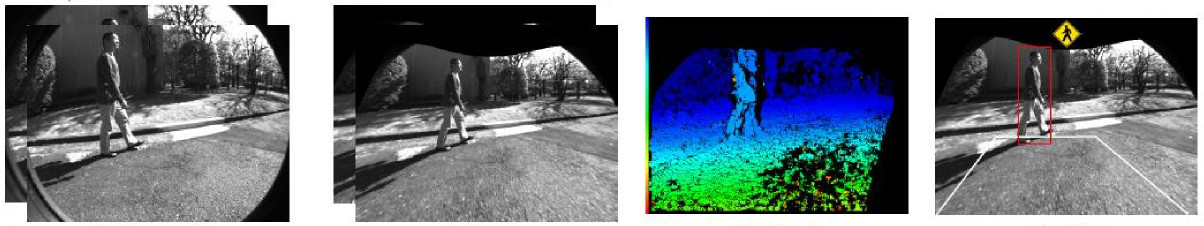
\includegraphics[width=10cm]{figures/car-pedestrian.jpg}}
    {\centering Image from Ryuzo Okada, Toyota}
\end{center}

\end{frame}

% -----------------------------------------------------------------------------

\begin{frame}
\frametitle{Person Detection}
\framesubtitle{Applications -- Interactive Art Installations}

\begin{center}
    \copyrightbox[b]
    {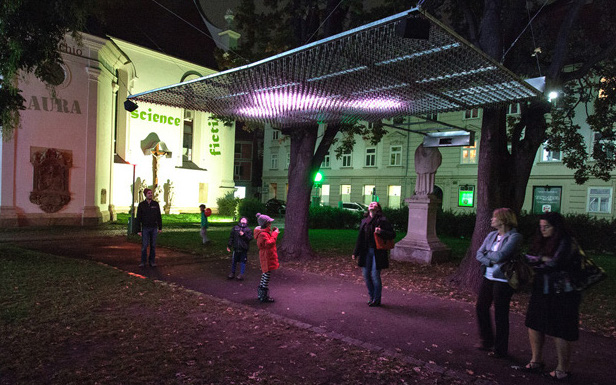
\includegraphics[width=8cm]{figures/ortlos-public-space.jpg}}
    {\centering Image from \url{ortlos.com}}
\end{center}

\end{frame}

% -----------------------------------------------------------------------------

\begin{frame}
\frametitle{Person Detection}
\framesubtitle{Applications -- Fall Detection (fearless)}

Fall detection system developed at CVL
\begin{itemize}
	\item Uses data from a single Kinect sensor
    \item Detects falls by tracking the height of persons
\end{itemize}

\bigskip
\begin{center}
    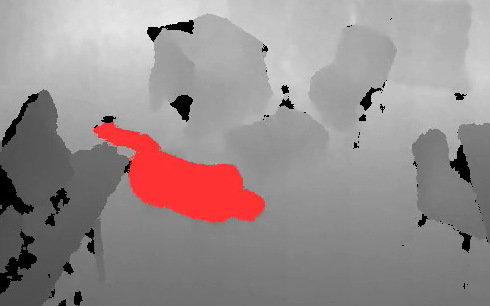
\includegraphics[width=6cm]{figures/fearless-screenshot.jpg}
\end{center}

\end{frame}

% -----------------------------------------------------------------------------

\begin{frame}
\frametitle{Person Detection}
\framesubtitle{Applications -- Entertainment (Kinect Player Pose Estimation)}

\begin{center}
    \url{https://www.youtube.com/watch?v=p2qlHoxPioM}
\end{center}

\begin{center}
    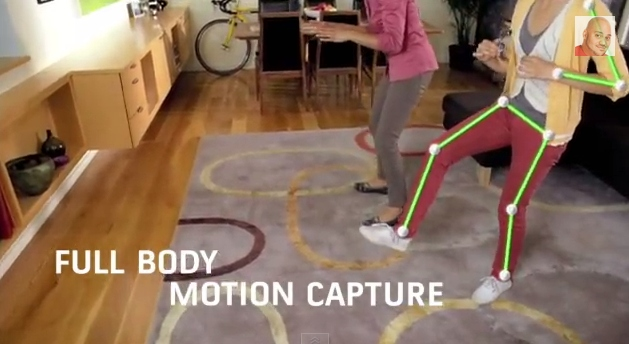
\includegraphics[width=8cm]{figures/kinect-promo.jpg}
\end{center}

\end{frame}

% -----------------------------------------------------------------------------

\begin{frame}
\frametitle{Kinect Player Pose Estimation}

Let's take a look at how this works\\\medskip
Assuming we have already detected the person

% this is Kinect v1's initial method, but Kinect v2 (and maybe later versions of v1 as well) work differently

\bigskip
\begin{center}
    \copyrightbox[b]
    {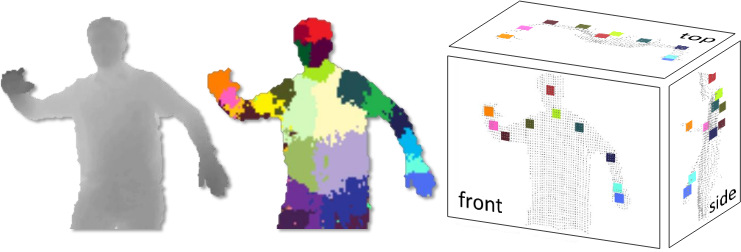
\includegraphics[width=8cm]{figures/kinect-pose.jpg}}
    {\centering Image from \cite{shotton2011}}
\end{center}

\end{frame}

% -----------------------------------------------------------------------------

\begin{frame}
\frametitle{Kinect Player Pose Estimation}
\framesubtitle{Steps}

Estimate body part of each pixel independently\\\medskip
Perform clustering to obtain joint position proposals\\\medskip
Fit skeleton model to joint proposals

\bigskip
\begin{center}
    \copyrightbox[b]
    {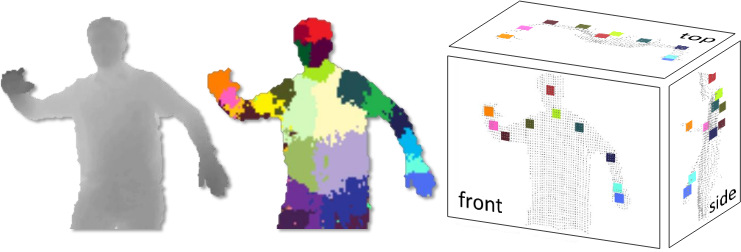
\includegraphics[width=8cm]{figures/kinect-pose.jpg}}
    {\centering Image from \cite{shotton2011}}
\end{center}

\end{frame}

% -----------------------------------------------------------------------------

\begin{frame}
\frametitle{Kinect Player Pose Estimation}
\framesubtitle{Pixel Classification}

For each pixel $\vx$ with depth $d(\vx)$ compute $\Pr(w|\vx)$ % depth as stored in depth map at pixel x, which corresponds to w in the previous slide set (i.e. not the Euclidean distance)
\begin{itemize}
     \item With $w$ representing the body part, $w\in\{0,\dots,30\}$ % these are shown below. note that the body side is important
     \item Note that this is a discriminative model % i.e. we infer a probability mass, not just a single hard label. refer to the models vs. algorithms slides
\end{itemize} 

\bigskip
\begin{center}
    \copyrightbox[b]
    {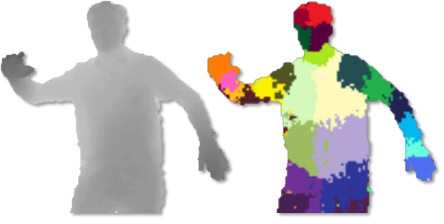
\includegraphics[width=5cm]{figures/kinect-pose-labels.jpg}}
    {\centering Image from \cite{shotton2011}}
\end{center}

\end{frame}

% -----------------------------------------------------------------------------

\begin{frame}
\frametitle{Kinect Player Pose Estimation}
\framesubtitle{Pixel Classification}

Classification using simple depth offset features $f_{\bth}$,
\[
    f_{\bth=(\vu,\vv)}(\vx)=d\left(\vx+\frac{\vu}{d(\vx)}\right)-d\left(\vx+\frac{\vv}{d(\vx)}\right)
\] % division by d(x) makes these features distance-invariant ... the offset adapts to d. also, these can be computed very quickly, which is required for real-time performance

\smallskip
\begin{center}
    \copyrightbox[b]
    {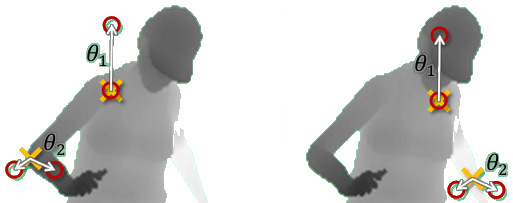
\includegraphics[width=7cm]{figures/kinect-pose-features.jpg}}
    {\centering Image adapted from \cite{shotton2011}} % here the yellow x denotes the current pixel and the two red pixels correspond to the locations used for offset computation. both features cause very different values in both images
\end{center}

\end{frame}

% -----------------------------------------------------------------------------

\begin{frame}
\frametitle{Kinect Player Pose Estimation}
\framesubtitle{Pixel Classification}

In isolation, one such feature $f_{\bth_1}$ is weak\\\medskip
But a strong classifier can be built by combining several features\\\medskip 
Method uses a forest of $T$ \emph{randomized decision trees} % this is only one example (but a powerful one) of an ensemble method, see Bishops book for more information

\bigskip
\begin{center}
    \copyrightbox[b]
    {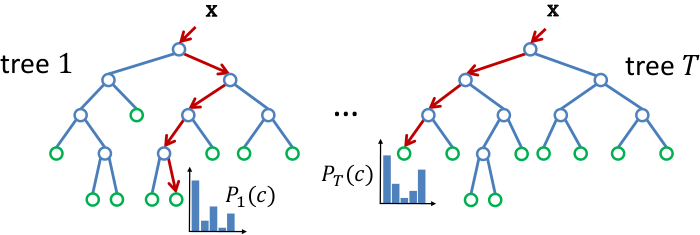
\includegraphics[width=8cm]{figures/kinect-pose-forest.png}}
    {\centering Image adapted from \cite{shotton2011}}
\end{center}

\end{frame}

% -----------------------------------------------------------------------------

\begin{frame}
\frametitle{Kinect Player Pose Estimation}
\framesubtitle{Pixel Classification -- Random Forests}

Each tree $t$ consist of split and leaf nodes\\\medskip
Each split node consists of a feature $f_{\bth}$ and a threshold $\tau$
\begin{itemize}
    \item $\vx$ branches down based on $f_{\bth_k}>\tau_k$
    \item Until a leaf node is reached, which stores $\Pr_t(w|\vx)$
\end{itemize}

\bigskip
Tree trained from training samples $(\vx,w)$ % extracted from different training images for each tree / for more information on how training works see "Randomized Trees for Real-Time Keypoint Recognition" by Lepetit et al.
\begin{itemize}
    \item $\bth_k,\tau_k$ selected randomly (hence random tree)
\end{itemize}

\bigskip
All trees contribute to result, $P(w|\vx)=\sum_{t=1}^T \Pr_t(w|\vx)$

\end{frame}

% -----------------------------------------------------------------------------

\begin{frame}[allowframebreaks=0.9]
\frametitle{Bibliography}

\printbibliography

\end{frame}

\end{document}
